\documentclass[11pt,a4paper,oneside]{article} % dock basic params

% Ru lang stuff
    \usepackage [utf8x] {inputenc}
    \usepackage [T2A] {fontenc}

% running titles 
    \usepackage{fancybox}
    \usepackage{fancyhdr}
    
% for last page number
    \usepackage{lastpage}

%for colored tablets cells
    \usepackage{colortbl}

% for Ru text in formulas
    \usepackage[warn]{mathtext}

% for captions 
    \usepackage[labelsep=period]{caption}

% for colored hyperrefs
    \usepackage{xcolor}
    \usepackage{hyperref}
    
% for pictures 
    \usepackage{graphicx}

% for coll math
    \usepackage{amsmath}

% path to all pictures
    \graphicspath{{picks/}}

% for enumerates
    \usepackage[shortlabels]{enumitem}

% for diff running titles on pages with diff parity
    \usepackage{ifthen}
    \usepackage{pdfpages}
    \usepackage[strict]{changepage}

%for drawings
    \usepackage{tikz}
    \usetikzlibrary{calc}
    \usetikzlibrary{decorations.pathmorphing}

% for good text in tablets
    \usepackage{array}
    \newcolumntype{P}[1]{>{\centering\arraybackslash}p{#1}}
    
% dock fields 20 15 15 35
    \usepackage[left=12mm, top=12mm, right=15mm, bottom=28mm, nohead, footskip=10mm]{geometry}
    
% for cool tables
    \usepackage{multirow}


% for different section/subsection/subsubsection styles in contents and doc

        \newcommand{\sect}[2] {
            \addtocounter{section}{1}
            \section*{\Huge\thesection.\,#1}
            \addcontentsline{toc}{subsection}{ \texorpdfstring{\thesection.\qquad\qquad #2}{Lg}}
        }
        
        \newcommand{\subsec}[2] {
            \addtocounter{subsection}{1}
            \subsection*{\thesubsection.\,#1}
            \addcontentsline{toc}{subsection}{ \texorpdfstring{\quad \thesubsection.\qquad\ #2}{Lg}}
        }
        
        \newcommand{\subsubsec}[2] {
            \addtocounter{subsubsection}{1}
            \subsubsection*{\thesubsubsection.\,#1}
            \addcontentsline{toc}{subsection}{ \texorpdfstring{\quad\quad\ \thesubsubsection. #2}{Lg}}
        }
%-------------------------------------------------------------------------%


% for easy mini pages with shifts
    \newcommand{\shiftedText}[3]{
    \hspace*{#1}\begin{minipage}[t]{#2}
        #3
    \end{minipage}
    }

% for lab number change in all doc
    \newcommand{\labnum}{
        2.5.1
    }

% page style setup (for running titles)
    \fancypagestyle{plain}{ %
    	\fancyhf{} % remove everything
    	
    	 % lines parameters
    	\renewcommand{\headrulewidth}{0pt}
    	\renewcommand{\footrulewidth}{0pt}
    	
    	% running titles contents
    	\fancyfoot[L]{\ifthenelse{\isodd{\thepage}}{Работа \labnum}{\thepage}}
    	\fancyfoot[R]{\ifthenelse{\isodd{\thepage}}{\thepage}{Работа \labnum}}
    }

% choosing page style with our running titles
    \pagestyle{plain}

\tolerance = 10000

% DOC BODY
\begin{document}
     % table of contents numeral depth
	    \setcounter{tocdepth}{4}
	
	% all counters setup
    	\setcounter{section}{0}
    	\setcounter{subsection}{0}
    	\setcounter{subsubsection}{0}
    	
    % some text placement parameters
    	\textheight = 240mm
    	\footskip = 10mm
        \leftskip = 10mm
    
    % add title page
    	
%!!! Just custom title stuff here !!!%

\shiftedText{0.5cm}{14cm}
{

    \begin{center}
    \vspace*{1.0cm}    
        
        {\bf\huge Работа \labnum }
        
    \vspace*{0.2cm}    
        
        {\bf\Large ИЗМЕРЕНИЕ ТЕПЛОПРОВОДНОСТИ ВОЗДУХА \\ ПРИ АТМОСФЕРНОМ ДАВЛЕНИИ }
        
    \vspace*{0.8cm}
        
        {\Large Работу выполнил Матренин Василий Б01-006 }
        
    \vspace*{1.6cm}
    
    \end{center}
    
    {\bf\noindent Цель работы: }  измерить коэффициент теплопроводности воздуха при атмосферном давлении в зависимости от температуры.
    
    \vspace*{0.6cm}
    
    {\bf\noindent В работе используются: } цилиндрическая колба с натянутой по оси нитью; термостат; вольтметр и амперметр (цифровые мультиметры); эталонное сопротивление; источник постоянного напряжения; реостат (или магазин сопротивлений).

}

\newpage
    	
    % fixing running titles shifts after title page
    	\headheight = 0.5cm
    	\headsep = 1.2cm
    
	% other file input
    	
%!!! Theoretical stuff here with all needed formulas (examples are here too) !!!%

% macro for comfortable numerated formula create 
    \newcommand{\formula}[3]
    {
        \noindent#1\\[0.1cm]
        \begin{equation}\label{#2}
            #3
        \end{equation}
    }

% macro for in-text math formulas
    \newcommand{\mth}[1]
    {
        \begin{math}
            #1
        \end{math}
    }

% macro for Russian-named indexes in formulas
    \newcommand{\ruB}[1]
    {
        _{\text{#1}}
    }

\section{\Large Теоритическая часть }

\noindent\hspace{1cm}Теплопроводность — это процесс передачи тепловой энергии от нагретых частей системы к холодным за счёт хаотического движения частиц среды (молекул, атомов и т.п.). В газах теплопроводность осуществляется за счёт непосредственной передачи кинетической энергии от быстрых молекул к медленным при их столкновениях. Перенос тепла описывается законом Фурье, утверждающим, что плотность потока энергии \mth{\overline{q} \left[ \frac{\text{Вт}}{\text{м}^2} \right]} (количество теплоты, переносимое через единичную площадку в единицу времени) пропорциональна градиенту температуры \mth{\nabla T}:

\formula
{}
{Fourier}
{\overline{q} = -k \cdot \nabla T,}

\noindentгде k\mth{\left[ \frac{\text{Вт}}{\text{м}\cdot K} \right]} - коэффициент теплопроводности. \\[0.2cm]

\noindent\hspace{1cm}Молекулярно-кинетическая теория даёт следующую оценку для коэффициента теплопроводности газов:

\formula
{}
{approxK}
{k \,\, \mathtt{\sim} \,\, \lambda \overline{v}\cdot nc_{_{V}},}

\noindentгде \mth{\lambda} - длинна свободного пробега молекул газа, \mth{\overline{v} = \sqrt{\frac{8k\ruB{Б}T}{\pi m}}} - средняя скорость их теплового движения, n - концентрация (объёмная плотность) газа, \mth{c_{_V} = \frac{i}{2}k\ruB{Б}} - его теплоемкость при постоянном объёме в расчёте на одну молекулу (i - эффективное число степеней свободы молекулы). \\[0.2cm]

\noindent\hspace{1cm}Длина свободного пробега может быть оценена как \mth{\lambda = \frac{1}{n\sigma}}, где \mth{\sigma} - эффектиное сечение столкновений молекул друг с другом. Тогда из (\ref{approxK}) видно, что коэффициент теплопроводности газа не зависит от плотности газа и определяется только его температурой. В простейшей модели твёрдых шариков \mth{\sigma = const}, и коэффициент теплопроводности пропорционален корню абсолютной температуры: \mth{k \propto \frac{\overline{v}}{\sigma} \propto \sqrt{T}}. На практике эффективное сечение \mth{\sigma(T)} следует считать медленно убывающей функцией T. \\[0.2cm]

\noindent\begin{minipage}[c]{0.54\textwidth}
    \hspace{1cm}Рассмотрим стационарную теплопроводность в цилиндрической геометрии (см. рис. 1). Пусть тонкая нить радиусом \mth{r_1} и длиной L помещена на оси цилиндра радиусом \mth{r_0.} Температура стенок цилиндра \mth{T_0} поддерживается постоянной. Пусть в нити выделяется некоторая тепловая мощность Q [Вт]. Если цилиндр длинный \mth{(L >> r_0),} можно пренебречь теплоотводом через его торцы. Тогда все параметры газа можно считать зависящими только от расстояния до оси системы r. Вместо (\ref{Fourier}) имеем:
\end{minipage}
\begin{minipage}[c]{0.4\textwidth}
    \begin{center}
        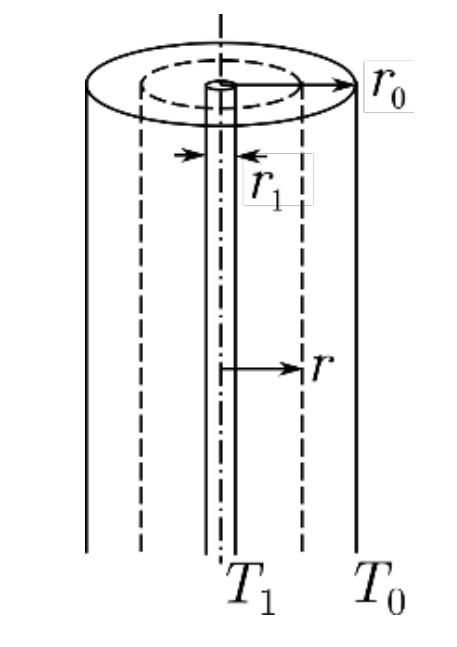
\includegraphics[scale=0.22]{picks/2_2_3_scheme1.jpg} \\
        \textit{\textcolor[HTML]{000000}{Рис. 1. Геометрия \\ задачи}}
    \end{center}
\end{minipage}

\formula
{}
{transFourier}
{q = -k\frac{dT}{dr}}

\newpage

\formula
{В стационарном состоянии полный поток тепла через любую цилиндрическую поверхность радиуса r площадью  \mth{S = 2\pi rL} должен быть одинаков и равен \mth{Q = qS}:}
{formQ}
{Q = -2\pi rL\cdot k\frac{dT}{dr} = const}

Если перепад температуры  \mth{\Delta T = T_1 - T_0} между нитью и стенками цилиндра мал \mth{(\Delta T << T_0),} то в (\ref{formQ}) можно пренебречь изменением теплопроводности от температуры в пределах системы, положив \mth{\chi \approx \chi(T_0)}. Тогда разделяя переменные в (\ref{formQ}) и интегрируя от радиуса нити до радиуса колбы получим:

\formula
{}
{finalQ}
{Q = \frac{2\pi L}{ln\frac{r_0}{r_1}} k\cdot \Delta T}

\vspace{1cm}

\begin{center}
    {\bf\Large
    Схема установки:}
    
    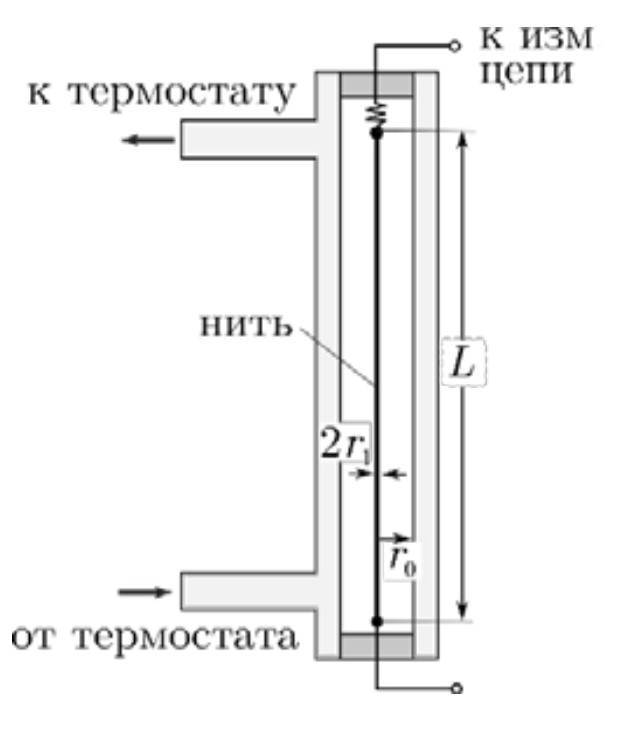
\includegraphics[scale=0.5]{picks/2_2_3_scheme2.jpg} \\
    \textit{\textcolor[HTML]{000000}{Рис. 2. Схема установки}}
    
\end{center}

\newpage
    	
\section{Ход работы}

\subsection{Проверка установки}
Проверил герметичность установки - успешно.

\subsection{Подбор частоты}
Подобрал частоту падения капель из аспиратора так, чтобы максимальное давление манометра не зависело от этой частоты (не чаще, чем 1 капля в 5 секунд).

\subsection{Максимальное давление спирта}

Измерил максимальное давление \mth{\Delta P\ruB{спирт}}  при  пробулькивании пузырьков воздуха через спирт.Пользуясь табличным значением коэффициента поверхностного натяжения спирта, определил по формуле (\ref{Laplas}) диаметр иглы. \\[0.2cm]

\noindent\mth{\Delta P\ruB{спирт} = 0000 \text{Па}} \\

\noindent\mth{\sigma^{\Delta P\ruB{спирт}} \ruB{случ} = 0000 \text{Па}} \\

\noindent\mth{d\ruB{иглы} = 0000 \text{мм}}

\subsection{Максимальное давление для поверхности воды}

Перенес предварительно промытую и просушенную от спирта иглу в колбу с дистиллированной водой. Измерил максимальное давление Р1 при пробулькивании пузырьков, когда игла лишь касается поверхности воды. Измерил расстояние между верхним концом иглы и !!! любой неподвижной частю !!! прибора h1. \\[0.2cm]

\noindent\mth{P1 = 0000\text{Па}} \\

\noindent\mth{h1 = 0000\text{м}}

\subsection{Максимальное давление на предельной глубине}

Утопил иглу до предела (между концом иглы и дном оставил небольшой зазор, чтобы образующийся пузырёк не касался дна). Измерил h2 (как в пункте 4).
Измерил максимальное давление в пузырьках Р2. По разности давлений \mth{\Delta P = P2 - P1} определил глубину погружения \mth{\Delta h} иглы и сравнил с \mth{\Delta h =  h1- h2}. 

\newpage

\mth{h2 = 0000\text{м}} \\

\mth{P2 = 0000\text{Па}} \\

\mth{\Delta P = 0000\text{Па}} \\

\mth{\Delta h = !!! = 0000\text{м}} \\

\mth{\Delta h = h1 - h2 = 0000\text{м}} \\

Значения \mth{\Delta h}, посчитаные разными способами, совпадают в пределах погрешностей.

\subsection {Зависимость $\sigma(T)$}

Снял зависимость $\sigma(T)$, результаты представлены в таблице 1.

\begin{table}[h!]
    \begin{center}
        \caption*{\color[HTML]{000000}Таблица 1: Зависимость $\sigma(T)$}
        \begin{tabular}{|| P{1.3cm}|P{1.3cm} || P{1.3cm}|P{1.3cm} || P{1.3cm}|P{1.3cm} || P{1.3cm}|P{1.3cm} ||} 
        \hline
        \hline

        \multicolumn{2}{||c||}{$ t = 25^\circ C$} & \multicolumn{2}{c||}{$ t = 30^\circ C$} & \multicolumn{2}{c||}{$ t = 35^\circ C$} & \multicolumn{2}{c||}{$ t = 40^\circ C$} \\

        \hline 
        
        P, Па & $\sigma, \frac{H}{m}$ & P, Па & $\sigma, \frac{H}{m}$ & P, Па & $\sigma, \frac{H}{m}$ & P, Па & $\sigma, \frac{H}{m}$ \\

        \hline

        0 & 0 & 0 & 0 & 0 & 0 & 0 & 0 \\
        \hline
        0 & 0 & 0 & 0 & 0 & 0 & 0 & 0 \\
        \hline

        \end{tabular}

        \vspace{0.5cm}

        \begin{tabular}{|| P{1.3cm}|P{1.3cm} || P{1.3cm}|P{1.3cm} || P{1.3cm}|P{1.3cm} ||} 
            \hline
            \hline

            \multicolumn{2}{||c||}{$ t = 45^\circ C$} & \multicolumn{2}{c||}{$ t = 50^\circ C$} & \multicolumn{2}{c||}{$ t = 55^\circ C$} \\

            \hline 

            P, Па & $\sigma, \frac{H}{m}$ & P, Па & $\sigma, \frac{H}{m}$ & P, Па & $\sigma, \frac{H}{m}$ \\

            \hline

            0 & 0 & 0 & 0 & 0 & 0 \\
            \hline
            0 & 0 & 0 & 0 & 0 & 0 \\
            \hline

            \end{tabular}

    \end{center}
\end{table}

    	%
%!!! Calculations result and graphs here !!!%

\subsection{График зависимостей R(Q)}

Построил график для зависимостей R(Q) при разных температурах. \\График представлен на Рис. 3. \\

\begin{center}
    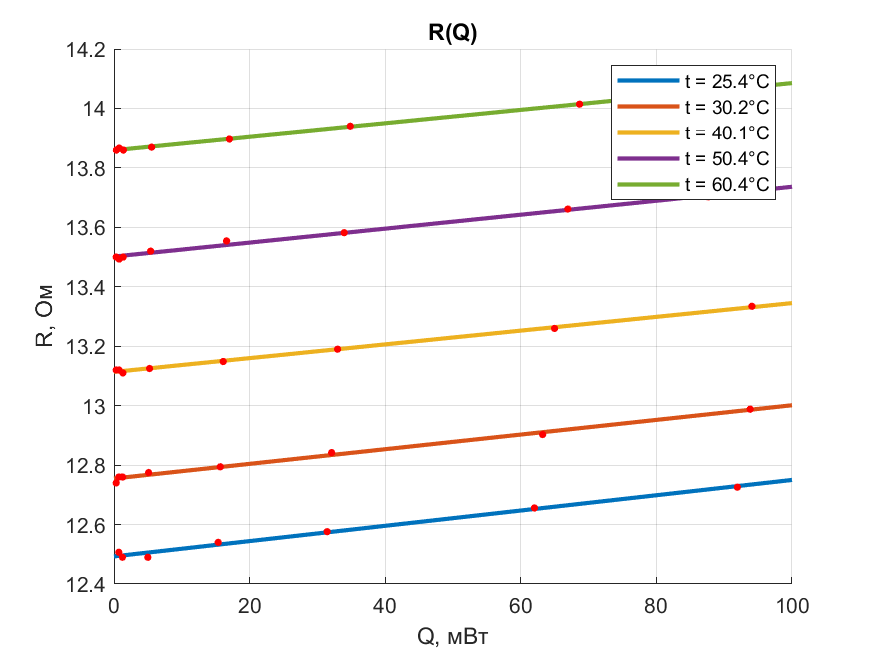
\includegraphics[scale = 1.3]{picks/223_R(Q).png} \\
    \textit{\textcolor[HTML]{000000}{Рис. 3. R(Q) для разных температур}}
\end{center}

\vspace{0.5cm}

    \begin{table}[h!]
    	\begin{center}
    		\caption*{\color[HTML]{000000}Таблица 2: Значения угловых к-тов \mth{\frac{dR}{dQ}} и значения R(0) для графика R(Q)}
    		\begin{tabular}{|P{3cm}|P{1.3cm}|P{1.3cm}|P{1.3cm}|P{1.3cm}|P{1.3cm}|}
    		\hline

                \mth{t, ^\circ C}    		& 25,4  & 30,2  & 40,1  & 50,4  & 60,4 \\  
    		    \hline
    		    R(0), Ом                    & 12,49 & 12,75 & 13,11 & 13,50 & 13,86 \\
    		    \hline
                \mth{\frac{dR}{dQ}, \frac{\text{Ом}}{\text{Вт}}}  & 2,57 & 2,46 & 2,31 & 2,34 & 2,25 \\


            \hline    		
    		\end{tabular}
    	\end{center}
    \end{table}

\newpage

\subsection{График зависимости R(t)}

Построил график для зависимости R(t). \\График представлен на Рис. 4. \\

\begin{center}
    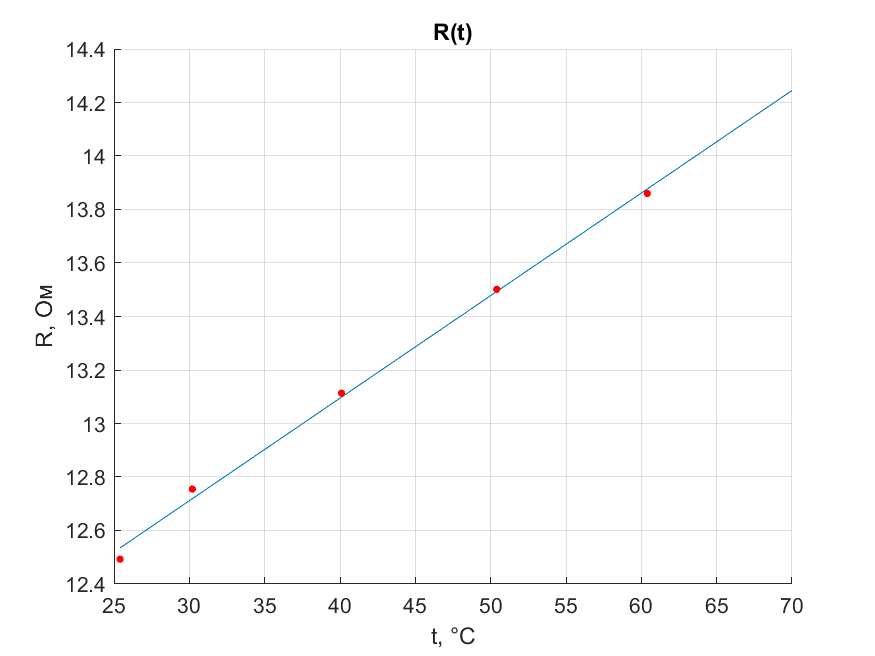
\includegraphics[scale = 1.3]{picks/223_R(T).png} \\
    \textit{\textcolor[HTML]{000000}{Рис. 4. R(t)}}
\end{center} 

\vspace{0.5cm}

Значение углового к-та для данного графика \mth{\frac{dR}{dT} = 3,83\cdot10^{-2} \frac{\text{Ом}}{K}}

\newpage

\subsection{Вычисление к-та теплопроводности при разных температурах термостата }

Из формулы (\ref{finalQ}) получил следующую формулу для расчета к: \\[0.2cm] 

\noindent\mth{k = \frac{\frac{dQ}{dR}\frac{dR}{dT}\,\cdot\, ln\frac{r_0}{r_1}}{2\pi L}} \\[0.2cm]

\noindent\mth{T_0} - Температура термостата; k - Значение теплопроводности. Результаты расчетов представлены в Таблице 3:

\begin{table}[h!]
    \begin{center}
        \caption*{\color[HTML]{000000}Таблица 3: к (T\mth{_0})}
        \begin{tabular}{|P{3cm}|P{1.3cm}|P{1.3cm}|P{1.3cm}|P{1.3cm}|P{1.3cm}|}
        \hline

            \mth{T_0, ^\circ C}    		         & 25,4  & 30,2  & 40,1  & 50,4  & 60,4 \\  
            \hline
            \mth{k, \frac{\text{Ом}}{\text{м}K} \cdot 10^{-2}} & 2,67 & 2,78 & 2,96 & 2,92 & 3,04 \\

        \hline    		
        \end{tabular}
    \end{center}
\end{table}

\subsection{График к(T)}

Пользуясь значениями из предыдущего пункта построил график к(T).\linebreak График представлен на рис. 5. \\

\begin{center}
    \includegraphics[scale = 1.0]{picks/223_k(T).png} \\
    \textit{\textcolor[HTML]{000000}{Рис. 5. k(t)}}
\end{center} 

\end{document}
